%!TEX program = xelatex

% 纸张模式:护眼模式-geye 朦胧模式-hazy
% 纸张尺寸:pad kindle pc normal screen
\documentclass[cn, blue, normal, 12pt]{elegantnote}

\title{自动控制原理笔记}
\author{Xiaohei}
\institute{Created by Elegant\LaTeX{}}
\version{0.1}
\date{\zhtoday}

\usepackage{pgfplots}
\pgfplotsset{compat=newest}
\usetikzlibrary{plotmarks}
\usetikzlibrary{arrows.meta}
\usepgfplotslibrary{patchplots}
\usepackage{grffile}
\usepackage{amsmath}
\usepackage{bm}
\usepackage{multirow}

\begin{document}

\maketitle

\section{控制系统的数学模型}

\subsection{线性控制系统}

\textbf{线性控制系统描述方法}

\begin{enumerate}
    \item 输入输出描述法(外部描述法):输入输出模型
    \item 状态空间描述法(内部描述法):状态空间模型
\end{enumerate}

\textbf{线性控制系统输入输出数学模型}

\begin{enumerate}
    \item 时域模型:微分方程
    \item 频域、复频域模型:传递函数
    \item 图示模型:方框图、信号流图
\end{enumerate}

\subsection{典型环节}

\subsubsection{惯性环节}

\begin{equation}
    G(s)=\frac{1}{Ts+1}
\end{equation}

其中$T$为惯性环节时间常数。

\subsubsection{积分环节}

\begin{equation}
    G(s)=\frac{1}{Ts}
\end{equation}

其中$T$为积分环节时间常数。

\subsubsection{振荡环节}

\begin{equation}
    G(s)=\frac{\omega_n^2}{s^2+2\zeta\omega_n s+\omega_n^2}=\frac{1}{T^2 s^2+2\zeta Ts+1}
\end{equation}

其中$T=\frac{1}{\omega_n}$为时间常数,$\zeta$为阻尼比,$\omega_n$为无阻尼自然振荡角频率。

\subsubsection{微分环节}

\begin{equation}
    G(s)=Ts
\end{equation}

其中$T$为微分环节时间常数。理想微分环节的传递函数不是真有理分式,工程实现较为困难,工程上常采用具有惯性环节的微分环节。

\subsubsection{比例环节}

\begin{equation}
    G(s)=K_p
\end{equation}

其中$K_p$为比例系数增益。

\subsubsection{时滞环节}

\begin{equation}
    G(s)=\text{e}^{-\tau s}
\end{equation}

其中$\tau$为延迟时间常数。

\subsection{框图模型}

框图的基本变换:合并串联方框、相加点前/后移、分支点前/后移、消去反馈回路。

负反馈控制系统的典型结构图:

\begin{center}
    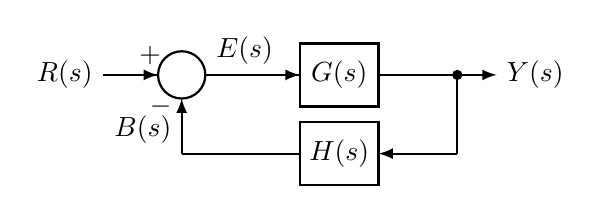
\begin{tikzpicture}[thick]
        \draw[-latex]     (2,2) -- (7,2);
        \draw[fill=white] (3,2) circle [radius=0.3];
        \draw[fill=white] (4.5,1.6) rectangle (5.5,2.4);
        \draw[fill=white] (4.5,0.6) rectangle (5.5,1.4);
        \draw[-latex]     (2,2)   -- (2.7,2);
        \draw[-latex]     (3.3,2) -- (4.5,2);
        \draw[-latex]     (6.5,1) -- (5.5,1);
        \draw[-latex]     (3,1)   -- (3,1.7);
        \draw             (6.5,2) -- (6.5,1);
        \draw             (4.5,1) -- (3,1);
        \filldraw         (6.5,2) circle [radius=0.05];
        \node[left]   at  (2,2)   {$R(s)$};
        \node[right]  at  (7,2)   {$Y(s)$};
        \node         at  (5,2)   {$G(s)$};
        \node         at  (5,1)   {$H(s)$};
        \node[above]  at  (3.8,2) {$E(s)$};
        \node[left]   at  (3,1.3) {$B(s)$};
        \node[above]  at  (2.6,2) {$+$};
        \node[left]   at  (3,1.6) {$-$};
    \end{tikzpicture}
\end{center}

闭环传递函数:

\begin{equation}
    \frac{Y(s)}{R(s)}=\frac{G(s)}{1+G(s)H(s)}
\end{equation}

前向传递函数:

\begin{equation}
    \frac{Y(s)}{E(s)}=G(s)
\end{equation}

开环传递函数:

\begin{equation}
    \frac{B(s)}{E(s)}=G(s)H(s)
\end{equation}

\section{控制系统的时域分析}

\subsection{线性定常系统}

线性定常系统的一个特性:系统对输入信号导数的响应,等于系统对该输入信号响应的导数;或者,系统对输入信号积分的响应,等于系统对该输入信号响应的积分,积分常数由零初始条件确定。

\subsection{状态空间方程的解}

系统状态空间方程为:

\begin{equation}
    \begin{aligned}
        \bm{\dot{x}}(t)&=\bm{Ax}(t)+\bm{Bu}(t) \\
        \bm{y}(t)&=\bm{Cx}(t)+\bm{Du}(t)
    \end{aligned}
\end{equation}

状态转移矩阵:

\begin{equation}
    \bm{\varPhi}(t)=\text{e}^{\bm{A}t}=\mathcal{L}^{-1}\left[(s\bm{I}-\bm{A})^{-1}\right]
\end{equation}

状态空间方程的解:

\begin{equation}
    \bm{x}(t)=\bm{\varPhi}(t)\bm{x}_0+\int_{0}^{t}\bm{\varPhi}(t-\tau)\bm{Bu}(\tau)\text{d}\tau
\end{equation}

系统的输出:

\begin{equation}
    y(t)=\bm{C\varPhi}(t)\bm{x}_0+\int_{0}^{t}\bm{C\varPhi}(t-\tau)\bm{Bu}(\tau)\text{d}\tau+\bm{Du}(t)
\end{equation}

单位阶跃响应:

\begin{equation}
    h(t)=-\bm{C}\bm{A}^{-1}\bm{B}+\bm{C}\bm{A}^{-1}\text{e}^{\bm{A}t}\bm{B}+\bm{D}
\end{equation}

静态放大系数:

\begin{equation}
    k_s=-\bm{C}\bm{A}^{-1}\bm{B}+\bm{D}
\end{equation}

\subsection{暂态性能指标}

延迟时间$T_d$:系统响应从0上升到稳态值的50\%所需要的时间

上升时间$T_r$:有振荡系统响应从0上升到稳态值所需时间;无振荡系统响应从稳态值的10\%上升到90\%所需时间。

峰值时间$T_p$:系统响应达到最大峰值所需要的时间。

最大超调量$\sigma\%$:系统响应超出稳态值的最大偏离量,常以百分比表示。

调节时间$T_s$:系统响应与稳态值之差达到误差$\pm\Delta$所需要的最小时间。

振荡次数$N$:调节时间$T_s$内,$y(t)$偏离$y(\infty)$的振荡次数。

\subsection{一阶系统的暂态响应特性}

一阶系统的闭环传递函数为:

\begin{equation}
    \frac{Y(s)}{R(s)}=\frac{1}{Ts+1}
\end{equation}

其单位阶跃响应如下:

\begin{figure}[htbp]
    \centering
    \caption{一阶系统单位阶跃响应}
    % This file was created by matlab2tikz.
%
%The latest updates can be retrieved from
%  http://www.mathworks.com/matlabcentral/fileexchange/22022-matlab2tikz-matlab2tikz
%where you can also make suggestions and rate matlab2tikz.
%
\definecolor{mycolor1}{rgb}{0.00000,0.44700,0.74100}%
%
\begin{tikzpicture}[scale=0.5]

\begin{axis}[%
width=4.396in,
height=3.357in,
at={(0.883in,0.481in)},
scale only axis,
separate axis lines,
every outer x axis line/.append style={white!40!black},
every x tick label/.append style={font=\color{white!40!black},scale=2},
every x tick/.append style={white!40!black},
xmin=0,
xmax=5,
xtick={0,1,2,3,4,5},
xticklabels={{$0$},{$T$},{$2T$},{$3T$},{$4T$},{$5T$}},
every outer y axis line/.append style={white!40!black},
every y tick label/.append style={font=\color{white!40!black},scale=2},
every y tick/.append style={white!40!black},
ymin=0,
ymax=1,
axis background/.style={fill=white},
xmajorgrids,
ymajorgrids
]
\addplot [color=mycolor1, forget plot]
  table[row sep=crcr]{%
0	0\\
0.0460517018598707	0.0450074139785543\\
0.0921034037197414	0.0879891606440716\\
0.138155105579612	0.129036410043893\\
0.184206807439483	0.168236228897295\\
0.230258509299353	0.205671765275678\\
0.276310211159224	0.24142242497077\\
0.322361913019095	0.275564039924958\\
0.368413614878966	0.308169029081007\\
0.414465316738836	0.339306551992343\\
0.460517018598707	0.369042655519742\\
0.506568720458578	0.397440413925574\\
0.552620422318448	0.424560062662772\\
0.598672124178319	0.450459126142302\\
0.64472382603819	0.475192539750152\\
0.69077552789806	0.498812766372651\\
0.736827229757931	0.521369907677283\\
0.782878931617802	0.542911810385045\\
0.828930633477672	0.563484167759754\\
0.874982335337543	0.583130616529583\\
0.921034037197414	0.601892829446421\\
0.967085739057285	0.619810603679357\\
1.01313744091716	0.636921945229817\\
1.05918914277703	0.653263149547387\\
1.1052408446369	0.668868878517327\\
1.15129254649677	0.683772233983081\\
1.19734424835664	0.698004827959718\\
1.24339595021651	0.711596849687259\\
1.28944765207638	0.724577129666104\\
1.33549935393625	0.736973200810383\\
1.38155105579612	0.748811356848964\\
1.42760275765599	0.760116708097974\\
1.47365445951586	0.770913234723147\\
1.51970616137573	0.78122383760497\\
1.5657578632356	0.791070386914523\\
1.61180956509547	0.80047376850304\\
1.65786126695534	0.809453928203605\\
1.70391296881522	0.818029914138932\\
1.74996467067509	0.826219917124994\\
1.79601637253496	0.834041309256177\\
1.84206807439483	0.841510680753823\\
1.8881197762547	0.848643875156315\\
1.93417147811457	0.855456022925345\\
1.98022317997444	0.86196157353965\\
2.02627488183431	0.868174326144299\\
2.07232658369418	0.874107458820525\\
2.11837828555405	0.879773556538201\\
2.16442998741392	0.885184637850256\\
2.21048168927379	0.890352180385627\\
2.25653339113366	0.895287145194857\\
2.30258509299353	0.899999999999948\\
2.34863679485341	0.904500741397806\\
2.39468849671328	0.90879891606436\\
2.44074019857315	0.912903641004344\\
2.48679190043302	0.916823622889686\\
2.53284360229289	0.920567176527526\\
2.57889530415276	0.924142242497037\\
2.62494700601263	0.927556403992458\\
2.6709987078725	0.930816902908064\\
2.71705040973237	0.933930655199199\\
2.76310211159224	0.936904265551941\\
2.80915381345211	0.939744041392526\\
2.85520551531198	0.942456006266247\\
2.90125721717185	0.945045912614201\\
2.94730891903172	0.947519253974987\\
2.9933606208916	0.949881276637238\\
3.03941232275147	0.952136990767703\\
3.08546402461134	0.95429118103848\\
3.13151572647121	0.956348416775952\\
3.17756742833108	0.958313061652936\\
3.22361913019095	0.960189282944621\\
3.26967083205082	0.961981060367915\\
3.31572253391069	0.963692194522962\\
3.36177423577056	0.96532631495472\\
3.40782593763043	0.966886887851715\\
3.4538776394903	0.968377223398291\\
3.49992934135017	0.969800482795955\\
3.54598104321004	0.97115968496871\\
3.59203274506991	0.972457712966595\\
3.63808444692978	0.973697320081024\\
3.68413614878966	0.974881135684883\\
3.73018785064953	0.976011670809784\\
3.7762395525094	0.977091323472302\\
3.82229125436927	0.978122383760485\\
3.86834295622914	0.979107038691441\\
3.91439465808901	0.980047376850293\\
3.96044635994888	0.98094539282035\\
4.00649806180875	0.981802991413883\\
4.05254976366862	0.98262199171249\\
4.09860146552849	0.983404130925608\\
4.14465316738836	0.984151068075373\\
4.19070486924823	0.984864387515623\\
4.2367565711081	0.985545602292526\\
4.28280827296797	0.986196157353957\\
4.32885997482785	0.986817432614422\\
4.37491167668772	0.987410745882045\\
4.42096337854759	0.987977355653813\\
4.46701508040746	0.988518463785019\\
4.51306678226733	0.989035218038556\\
4.5591184841272	0.989528714519479\\
4.60517018598707	0.989999999999988\\
4.65122188784694	0.990450074139774\\
4.69727358970681	0.99087989160643\\
4.74332529156668	0.991290364100429\\
4.78937699342655	0.991682362288963\\
4.83542869528642	0.992056717652747\\
4.88148039714629	0.992414224249699\\
4.92753209900616	0.992755640399241\\
4.97358380086604	0.993081690290802\\
};
\end{axis}

\end{tikzpicture}%

\end{figure}

延迟时间$T_d$:

\begin{equation}
    T_d=-T\ln{0.5}=0.69T
\end{equation}

上升时间$T_r$:

\begin{equation}
    T_r=(-T\ln{0.9})-(-T\ln{0.1})=2.20T
\end{equation}

\subsection{二阶规范系统的暂态响应特性}

二阶规范系统的闭环传递函数为:

\begin{equation}
    \frac{Y(s)}{R(s)}=\frac{\omega_n^2}{s^2+2\zeta\omega_n s+\omega_n^2}
\end{equation}

其中$\zeta$为阻尼比,$\omega_n$为无阻尼自然振荡角频率。
$\zeta$的值影响系统的响应情况如下表所示。

\begin{table}[htbp]
    \label{tab:zeta}
    \begin{center}
      \caption{$\zeta$的值对系统响应影响}
      \begin{tabular}{c|c|c|c|c|c}
        \hline
        $\bm{\zeta}$ & $\zeta<0$ & $\zeta=0$ & $0<\zeta<1$ & $\zeta=1$ & $\zeta>1$ \\
        \hline
        \textbf{状态} & 不稳定 & 无阻尼 & 欠阻尼 & 临界阻尼 & 过阻尼 \\
        \hline
        \textbf{响应} & - & 无衰减振荡 & 衰减振荡 & 无振荡 & 无振荡 \\
        \hline
      \end{tabular}
    \end{center}
\end{table}

欠阻尼或临界阻尼时:

\begin{equation}
    -p_{1,2}=-\zeta\omega_n\pm\text{j}\omega_n\sqrt{1-\zeta^2}=\sigma\pm\text{j}\omega_d
\end{equation}

其中,$\omega_d=\omega_n\sqrt{1-\zeta^2}$为阻尼自然振荡角频率,$\sigma=-\zeta\omega_n$为阻尼系数或衰减系数。

过阻尼时:

\begin{equation}
    -p_{1,2}=-\zeta\omega_n\pm\omega_n\sqrt{\zeta^2-1}
\end{equation}

峰值时间$T_p$:

\begin{equation}
    T_p=\frac{\pi}{\omega_d}=\frac{\pi}{\omega_n\sqrt{1-\zeta^2}}
\end{equation}

超调量$\sigma\%$:

\begin{equation}
    \sigma\%=\text{e}^{-\frac{\zeta\pi}{\sqrt{1-\zeta^2}}}\times 100\%
\end{equation}

上升时间$T_r$:

\begin{equation}
    T_r=\frac{\pi-\varphi}{\omega_d}=\frac{\pi-\varphi}{\omega_n\sqrt{1-\zeta^2}} \quad \varphi=\arctan{\frac{\sqrt{1-\zeta^2}}{\zeta}}
\end{equation}

调节时间$T_s(0<\zeta<0.9)$:

\begin{equation}
    T_s(2\%)=\frac{4}{\zeta\omega_n} \quad T_s(5\%)=\frac{3}{\zeta\omega_n}
\end{equation}

二阶工程最佳参数:

\begin{equation}
    \zeta=\frac{1}{\sqrt{2}} \quad \sigma\%=\text{e}^{-\pi}\times 100\%=4.3\%
\end{equation}

添加零点对原无零点规范二阶系统性能的影响:峰值时间提前、超调量增大(振荡加剧)、调节时间增长。

\subsection{控制系统的稳态误差}

开环传递函数$G(s)$中零极点的重数$N$,即串联的积分环节的个数,称为系统的类型或阶数。

单位反馈系统的误差系数与稳态误差的定义:

\begin{equation}
    K=\lim_{s\rightarrow 0}G(s)=\lim_{s\rightarrow 0}\frac{K}{s^N} \quad e_{ss}=\lim_{s\rightarrow 0}E(s)=\lim_{s\rightarrow 0}\frac{A}{1+G(s)}
\end{equation}

单位反馈系统的误差系数与稳态误差如下表:

\begin{table}[htbp]
    \label{tab:zeta}
    \begin{center}
      \caption{系统的误差系数与稳态误差}
      \begin{tabular}{c|c|c|c|c|c|c}
        \hline
        \multirow{2}*{系统的类型} & \multicolumn{3}{|c|}{误差系数} & \multicolumn{3}{|c}{稳态误差} \\
        \cline{2-7}
        ~ & $K_p$ & $K_v$ & $K_a$ & $e_{ss}=A/(1+K_p)$ & $e_{ss}=A/K_v$ & $e_{ss}=A/K_a$ \\
        \hline
        0型 & $K$ & $0$ & $0$ & $A/(1+K)$ & $\infty$ & $\infty$ \\ 
        \hline
        1型 & $\infty$ & $K$ & $0$ & $0$ & $A/K$ & $\infty$ \\ 
        \hline
        2型 & $\infty$ & $\infty$ & $K$ & $0$ & $0$ & $A/K$ \\ 
        \hline
      \end{tabular}
    \end{center}
\end{table}

分析非单位反馈系统的稳态误差时,开环传递函数等效为:

\begin{equation}
    G_k(s)=G(s)H(s)
\end{equation}

\subsection{控制系统的稳定性}

稳定系统:对于有界输入具有有界响应。

充要条件:系统传递函数的所有极点(系统矩阵的特征值)具有负实部(在$s$平面虚轴左面)。

稳定性判据:Routh-Hurwitz稳定性判据。

系统稳定的必要条件:特征方程的各项系数均为正(同号且不缺项)。

系统稳定的充分必要条件:Routh表中第一列各值为正。

\section{根轨迹法}



\end{document}
